%% This is file `elsarticle-template-1-num.tex',
%%
%% Copyright 2009 Elsevier Ltd
%%
%% This file is part of the 'Elsarticle Bundle'.
%% ---------------------------------------------
%%
%% It may be distributed under the conditions of the LaTeX Project Public
%% License, either version 1.2 of this license or (at your option) any
%% later version.  The latest version of this license is in
%%    http://www.latex-project.org/lppl.txt
%% and version 1.2 or later is part of all distributions of LaTeX
%% version 1999/12/01 or later.
%%
%% The list of all files belonging to the 'Elsarticle Bundle' is
%% given in the file `manifest.txt'.
%%
%% Template article for Elsevier's document class `elsarticle'
%% with numbered style bibliographic references
%%
%% $Id: elsarticle-template-1-num.tex 149 2009-10-08 05:01:15Z rishi $
%% $URL: http://lenova.river-valley.com/svn/elsbst/trunk/elsarticle-template-1-num.tex $
%%

%\documentclass[preprint,authoryear,review,12pt]{elsarticle}
\documentclass[final,5p,times,twocolumn]{elsarticle}

%% Use the option review to obtain double line spacing
%% \documentclass[preprint,review,12pt]{elsarticle}

%% Use the options 1p,two column; 3p; 3p,twocolumn; 5p; or 5p,twocolumn
%% for a journal layout:
%% \documentclass[final,1p,times]{elsarticle}
%% \documentclass[final,1p,times,twocolumn]{elsarticle}
%% \documentclass[final,3p,times]{elsarticle}
%% \documentclass[final,3p,times,twocolumn]{elsarticle}
%% \documentclass[final,5p,times]{elsarticle}
%% \documentclass[final,5p,times,twocolumn]{elsarticle}


\usepackage{color}
\usepackage{multirow,booktabs,ctable,array}
\usepackage{lscape}
\usepackage{amsmath}
\usepackage{lineno}
\usepackage{ulem}
\usepackage{setspace}
\usepackage{listings}
\usepackage{float}


\floatstyle{plain}
\newfloat{command}{thp}{lop}
\floatname{command}{Command}

%\usepackage[nomarkers,notablist]{endfloat}

%% if you use PostScript figures in your article
%% use the graphics package for simple commands
%% \usepackage{graphics}
%% or use the graphicx package for more complicated commands
%% \usepackage{graphicx}
%% or use the epsfig package if you prefer to use the old commands
%% \usepackage{epsfig}

%% The amssymb package provides various useful mathematical symbols
\usepackage{amssymb}
%% The amsthm package provides extended theorem environments
% \usepackage{amsthm}
 
 \usepackage{makecell}

%% The lineno packages adds line numbers. Start line numbering with
%% \begin{linenumbers}, end it with \end{linenumbers}. Or switch it on
%% for the whole article with \linenumbers after \end{frontmatter}.
%% \usepackage{lineno}

%% natbib.sty is loaded by default. However, natbib options can be
%% provided with \biboptions{...} command. Following options are
%% valid:

%%   round  -  round parentheses are used (default)
%%   square -  square brackets are used   [option]
%%   curly  -  curly braces are used      {option}
%%   angle  -  angle brackets are used    <option>
%%   semicolon  -  multiple citations separated by semi-colon
%%   colon  - same as semicolon, an earlier confusion
%%   comma  -  separated by comma
%%   numbers-  selects numerical citations
%%   super  -  numerical citations as superscripts
%%   sort   -  sorts multiple citations according to order in ref. list
%%   sort&compress   -  like sort, but also compresses numerical citations
%%   compress - compresses without sorting
%%
%% \biboptions{comma,round}

% \biboptions{}

\providecommand{\OO}[1]{\operatorname{O}\bigl(#1\bigr)}

\graphicspath{{./Figures/}
                          }

\long\def\symbolfootnote[#1]#2{\begingroup%
\def\thefootnote{\fnsymbol{footnote}}\footnote[#1]{#2}\endgroup}

    \usepackage{color}

    \definecolor{listcomment}{rgb}{0.0,0.5,0.0}
    \definecolor{listkeyword}{rgb}{0.0,0.0,0.5}
    \definecolor{listnumbers}{gray}{0.65}
    \definecolor{listlightgray}{gray}{0.955}
    \definecolor{listwhite}{gray}{1.0}

\newcommand{\lstsetcpp}
{
\lstset{frame = tb,
        framerule = 0.25pt,
        float,
        fontadjust,
        backgroundcolor={\color{listlightgray}},
        basicstyle = {\ttfamily\scriptsize},
        keywordstyle = {\ttfamily\color{listkeyword}\textbf},
        identifierstyle = {\ttfamily},
        commentstyle = {\ttfamily\color{listcomment}\textit},
        stringstyle = {\ttfamily},
        showstringspaces = false,
        showtabs = false,
        numbers = none,
        numbersep = 6pt,
        numberstyle={\ttfamily\color{listnumbers}},
        tabsize = 2,
        language=[ANSI]C++,
        floatplacement=!h,
        caption={\small {\ttfamily CreateDTICohort} which implements the a ground truth DTI simulator \cite{van-hecke2009}.  The short command line menu which is invoked using the  `{\ttfamily {-}h}'  option.  The long command line menu is obtained by typing `{\ttfamily {-}{-}help}'},
        captionpos=b,
        }
}




\journal{Neuroimage}

\begin{document}


\begin{frontmatter}

\title{Circularity in Voxel-Based Analysis}



\author[label1]{Nicholas J.~Tustison\fnref{label0}}
%  \ead{ntustison@virginia.edu}
  \fntext[label0]{\scriptsize Corresponding author:  PO Box 801339, Charlottesville, VA 22908; T:  434-924-7730; email address:  ntustison@virginia.edu }
\author[label2]{Brian B.~Avants}
\author[label2]{Philip A.~Cook}
\author[label3]{Junghoon Kim}
\author[label3]{John Whyte}
\author[label2]{James C.~Gee}
\author[label1]{James R.~Stone}

\address[label1]{Department of Radiology and Medical Imaging, University of Virginia, Charlottesville, VA}
\address[label2]{Penn Image Computing and Science Laboratory, University of Pennsylvania,
                Philadelphia, PA}
\address[label3]{Moss Rehabilitation Research Institute, Albert Einstein Healthcare Network, Philadelphia, PA}



%\maketitle

%\linenumbers


\begin{abstract}
Recent discussions within the neuroimaging community have highlighted the
problematic presence of selection bias in experimental design.  Although 
initially centering around the selection of voxels during the course of
fMRI studies, we demonstrate how this concept of circularity bias can 
potentially corrupt voxel-based analyses with a particular emphasis on
population studies of fractional anisotropy (FA).  
For such studies, template-based registration plays a critical role
in which a representative template serves as the normalized space for 
group alignment.  Following 
computation of FA, each subject's FA map is registered to the FA template prior to 
performing statistical comparisons between different groups within a population.
We illustrate how this analysis strategy can induce selection
bias which varies in strength with the similarity metric used in
registration.  Specifically, we show that the popular sum of squared
difference intensity metric  maximizes effect size, rather than
anatomical alignment, and consistently overestimates statistical
significance.  Consequently, we advocate a more cautious approach
that normalizes a population of FA images through the associated 
anatomical images.  One possibility, the Symmetric Group Normalization
strategy for unbiased template construction from anatomical (e.g.
T1-weighted) images, provides a valid and unbiased coordinate system for
statistical inference of FA differences.  
We establish this
outcome by using simulated data derived from normal controls from the International
Neuroimaging Data-sharing Initiative as well as a cohort of 16 traumatic
brain injury survivors compared with 17 control subjects.  
Alignment
comparisons with the normalization component of the popular tract-based
spatial statistics (TBSS) show that our anatomically-based template
approach produces good alignments despite the absence of any direct
FA-to-FA registration.  
%Of practical consideration we note that the
%software tools discussed in this work are provided to the public as part
%of the open source Advanced Normalization Tools (ANTs) repository.  
In conclusion, we recommend against circular analysis strategies that 
select image similarity metrics that are tied directly to the statistical 
functions used to assess population effects. 
\end{abstract}

\begin{keyword}
Advanced Normalization Tools (ANTs) \sep circularity\ diffusion tensor imaging \sep fractional anisotropy \sep template construction \sep voxel-based analysis
%% keywords here, in the form: keyword \sep keyword
\end{keyword}

\end{frontmatter}
%
%
\newpage


%% MSC codes here, in the form: \MSC code \sep code
%% or \MSC[2008] code \sep code (2000 is the default)

%%
%% Start line numbering here if you want
%%
% \linenumbers

%% main text

\section{Introduction}
Motivating the findings of a recent paper, the authors related their
puzzlement at the unusually high number of papers reporting 
significant correlations in fMRI studies \cite{Vul2009}. During the 
resulting investigation, the authors discovered the permeating
presence of a particular bias characterized by such related terms as ``circularity''
and ``non-independence''.
While related literature has focused on the presence of such bias in 
fMRI studies \cite{Vul2009,Vul2010} and, more generally, in neuroscience research 
\cite{Kriegeskorte2009}, we show how this can potentially extend to what has
become a fundamental neuroimaging analysis technique---voxel-based analysis.

Similarly, we were perplexed by the disparity in statistical results of one of 
our recent analyses \cite{Stone2011} using the same DTI data and same 
voxel-based analysis technique but different normalization approaches.  Despite 
distinctively better alignments with one approach, there was little 
difference in the statistical results between the two approaches.  
It was eventually discovered that the 
incommensurability between alignment quality and effect size in our
analysis was also a due to a subtle, yet significant circularity bias
which we explain below in the context of FA population studies.  
%Due to the public availability and widespread use of
%these voxel-based analysis tools we show 
%how this source of bias can enter into voxel-based studies focusing on
%population-based FA .

%Whereas the authors
%of \cite{Vul2009} were able to estimate reliability measures of
%both personality tests and fMRI and, thus, provide an upper bound 
%for possible correlations, the nature of the the analysis provided
%no indication as to the source of the disparity.


%State the objectives of the work and provide an adequate background, avoiding a detailed literature survey or a summary of the results.

The seminal work of Basser et al. \citep{Basser1994a,Basser1994} established diffusion tensor imaging (DTI) as a viable investigatory MRI technique.  DTI's sensitivity to brain architecture \citep{Basser1996,Assaf2008} enables promising analysis possibilities assessing neuro-structural differences in cross-population studies \citep{Kubicki2005,Arnone2008,Kantarci2010,Rametti2010}.
% including subjects with traumatic brain injury (TBI) \citep{Caeyenberghs2010,Jiang2010,Warner2010}.  
Two popular comprehensive software packages for assessing population FA differences include the SPM Matlab-based toolkit%
\footnote{
http://www.fil.ion.ucl.ac.uk/spm/
}
for voxel-based morphometry (VBM)
and the tract-based spatial statistics (TBSS) framework \citep{Smith2006}.%
\footnote{
http://www.fmrib.ox.ac.uk/fsl/tbss/index.html
} 
VBM \citep{Ashburner2001} continues to find application to FA studies \citep{Kakeda2010,Takao2010,Preziosa2011} despite concerns about its general validity \citep{Bookstein2001,Davatzikos2004} and with respect to DTI \citep{Jones2005,Chung2008}.  The TBSS framework was partially developed in response to these concerns in which voxel values are projected onto a template white matter skeleton for increased statistical power.  
%(e.g. \citep{Arnone2008,Bodini2009}).  

Although there are substantive differences in normalization
between these and other analysis approaches, a core
commonality includes direct FA-to-FA registration using various similarity metrics.  The sum of squared differences (SSD) image similarity metric is perhaps the easiest to interpret (it drives the image intensity difference to zero), is computationally efficient (just compute the image difference and gradient), and is therefore widely used.  Some of the most popular registration methods (e.g. SPM, 
Demons \cite{Thirion1998}, FSL's FNIRT, AIR \citep{Woods1998}, and LDDMM \citep{Beg2005}) rely on this metric and yield reasonable performance levels \citep{Klein2009}.%
%\footnote{
%In addition to TBSS and SPM, other popular packages in the neuroimaging community 
%which use the SSD metric include AIR \citep{Woods1998} and LDDMM \citep{Beg2005}.
%}  

However, suppose the SSD metric is used to find a set of $M$ transformations that map a population of $M$ FA images, $\{I_1, I_2, \ldots, I_M\}$, to a representative FA template, $J$, for statistical testing between groups. This results in the transformations,
$\boldsymbol{\mathcal{T}} = \{\mathcal{T}_1, \mathcal{T}_2,\ldots,\mathcal{T}_M \}$, which minimize the SSD metric over the population, i.e.
\begin{align}
  \boldsymbol{\mathcal{T}} = \underset{\mathcal{T}_1, \ldots, \mathcal{T}_M}{\operatorname{argmin}}
    \sum_{m=1}^M\sum_{n=1}^N \left( I^n_m( \mathcal{T}_m(\mathbf{x}) ) - J \right)^2.
\end{align}
Switching the order of the summations (since the transformations are mutually independent) and recognizing that a principal criterion for the selection of $J$ is such that it be a good approximation of the mean of the aligned images, it becomes apparent that the transformation solution
\begin{align}\label{eq:variance}
  \boldsymbol{\mathcal{T}} = \underset{\mathcal{T}_1, \ldots, \mathcal{T}_M}{\operatorname{argmin}}
    \sum_{n=1}^N \underbrace{\sum_{m=1}^M \left( I^n_m( \mathcal{T}_m(\mathbf{x}) ) - J \right)^2}_{
    \propto\mathrm{\,voxelwise\,variance}}
\end{align}
is that which minimizes the voxelwise group variance, or at least an approximation thereof.  Reducing the group variance will also directly affect the value of a standard population statistic, the Student's $t$-test.  Other standard similarity metrics will also exhibit this
trend to some degree as they minimize some local measure of intensity-based distance between the subject and the template.  

Thus, instead of normalization based on anatomical alignment followed by
statistical testing, direct normalization of the images to be statistically compared 
explicitly conflates
anatomical alignment with optimizing the very statistical testing
results that one will ultimately use to assess hypotheses.  This immediately evokes a sense of circularity in the analysis \citep{Kriegeskorte2010}.
According to Kriegeskrote et al., ``An analysis is circular (or nonindependent) if it is based on data that were selected for showing the effect of interest or a related effect.''  As illustrated with
Eqn. \ref{eq:variance}, direct FA-to-FA template registration will produce transformations that align (or select) voxels such that the statistical testing result (or the effect of interest) is increased (assuming one is using Student's 
$t$-test).  While the SSD metric is able to provide visually attractive alignments across subjects, the voxel-level details (that is, which voxels are matched where) are strikingly important in terms of the effect on detection power.  



Although various processing choices mitigate the effects of such bias,
such as Gaussian smoothing, nonparametric testing \citep{Rorden2007}, 
statistical analysis based on orthogonal projections onto the white matter skeleton 
\cite{Smith2006}, multiple comparisons corrections \cite{Nichols2003}, and the use of more robust similarity metrics, 
such choices are often made ad hoc and/or post hoc and, to our 
knowledge, not with the realization of the potential
for circularity bias described by Eqn. (\ref{eq:variance}).  

Instead of direct FA-to-FA template mapping for 
alignment to the normalized space, we advocate a statistically 
independent alignment protocol in which the FA images are mapped to 
the common reference space via intra-subject FA-to-T1 mapping 
followed by T1-to-T1 template alignment thus eliminating all direct
FA-to-FA registrations. The key point is that the intensity value differences used 
to assess alignment (i.e. the similarity metric) in FA-to-T1 and T1-to-T1 
normalizations are statistically independent of the intensity value differences used for 
the post-alignment numerical analysis.  It should be noted that this discussion
is certainly not limited to studies involving FA.  From 
Eqn. (\ref{eq:variance}), it is evident that such bias can occur anytime the 
similarity metric (and the values employed) are non-independent of 
the statistical analysis. 

Using simulated data, we first establish that this effect is real 
and warrants concern on the part of researchers using 
these techniques.  We then show how the general application
of a high performance \citep{Klein2009}, nonrigid registration algorithm 
\citep{Avants2011}, which forms the underlying machinery for an optimal 
template construction algorithm \citep{Avants2010}, can facilitate alignment 
between DTI-derived scalar images for cross-population studies.  
Although this type of alignment procedure is not uncommon 
(e.g. \cite{Lipton2008}), to our knowledge, this is the 
first time a connection has been made with the concept of 
circularity.  

%The rest of the paper establishes the severity of 
%this bias in situations
% although scientific best 
%practices would dictate the reasonable removal of all 
%potential sources of bias (including circularity) regardless of 
%the general degree of severity. 








\section{Methods and Materials}
% Provide sufficient detail to allow the work to be reproduced. 
% Methods already published should be indicated by a reference: 
% only relevant modifications should be described.

\subsection{Template Construction for Anatomically-Based Population Normalization}

\begin{figure*}
\begin{center}
\begin{tabular}{c}
  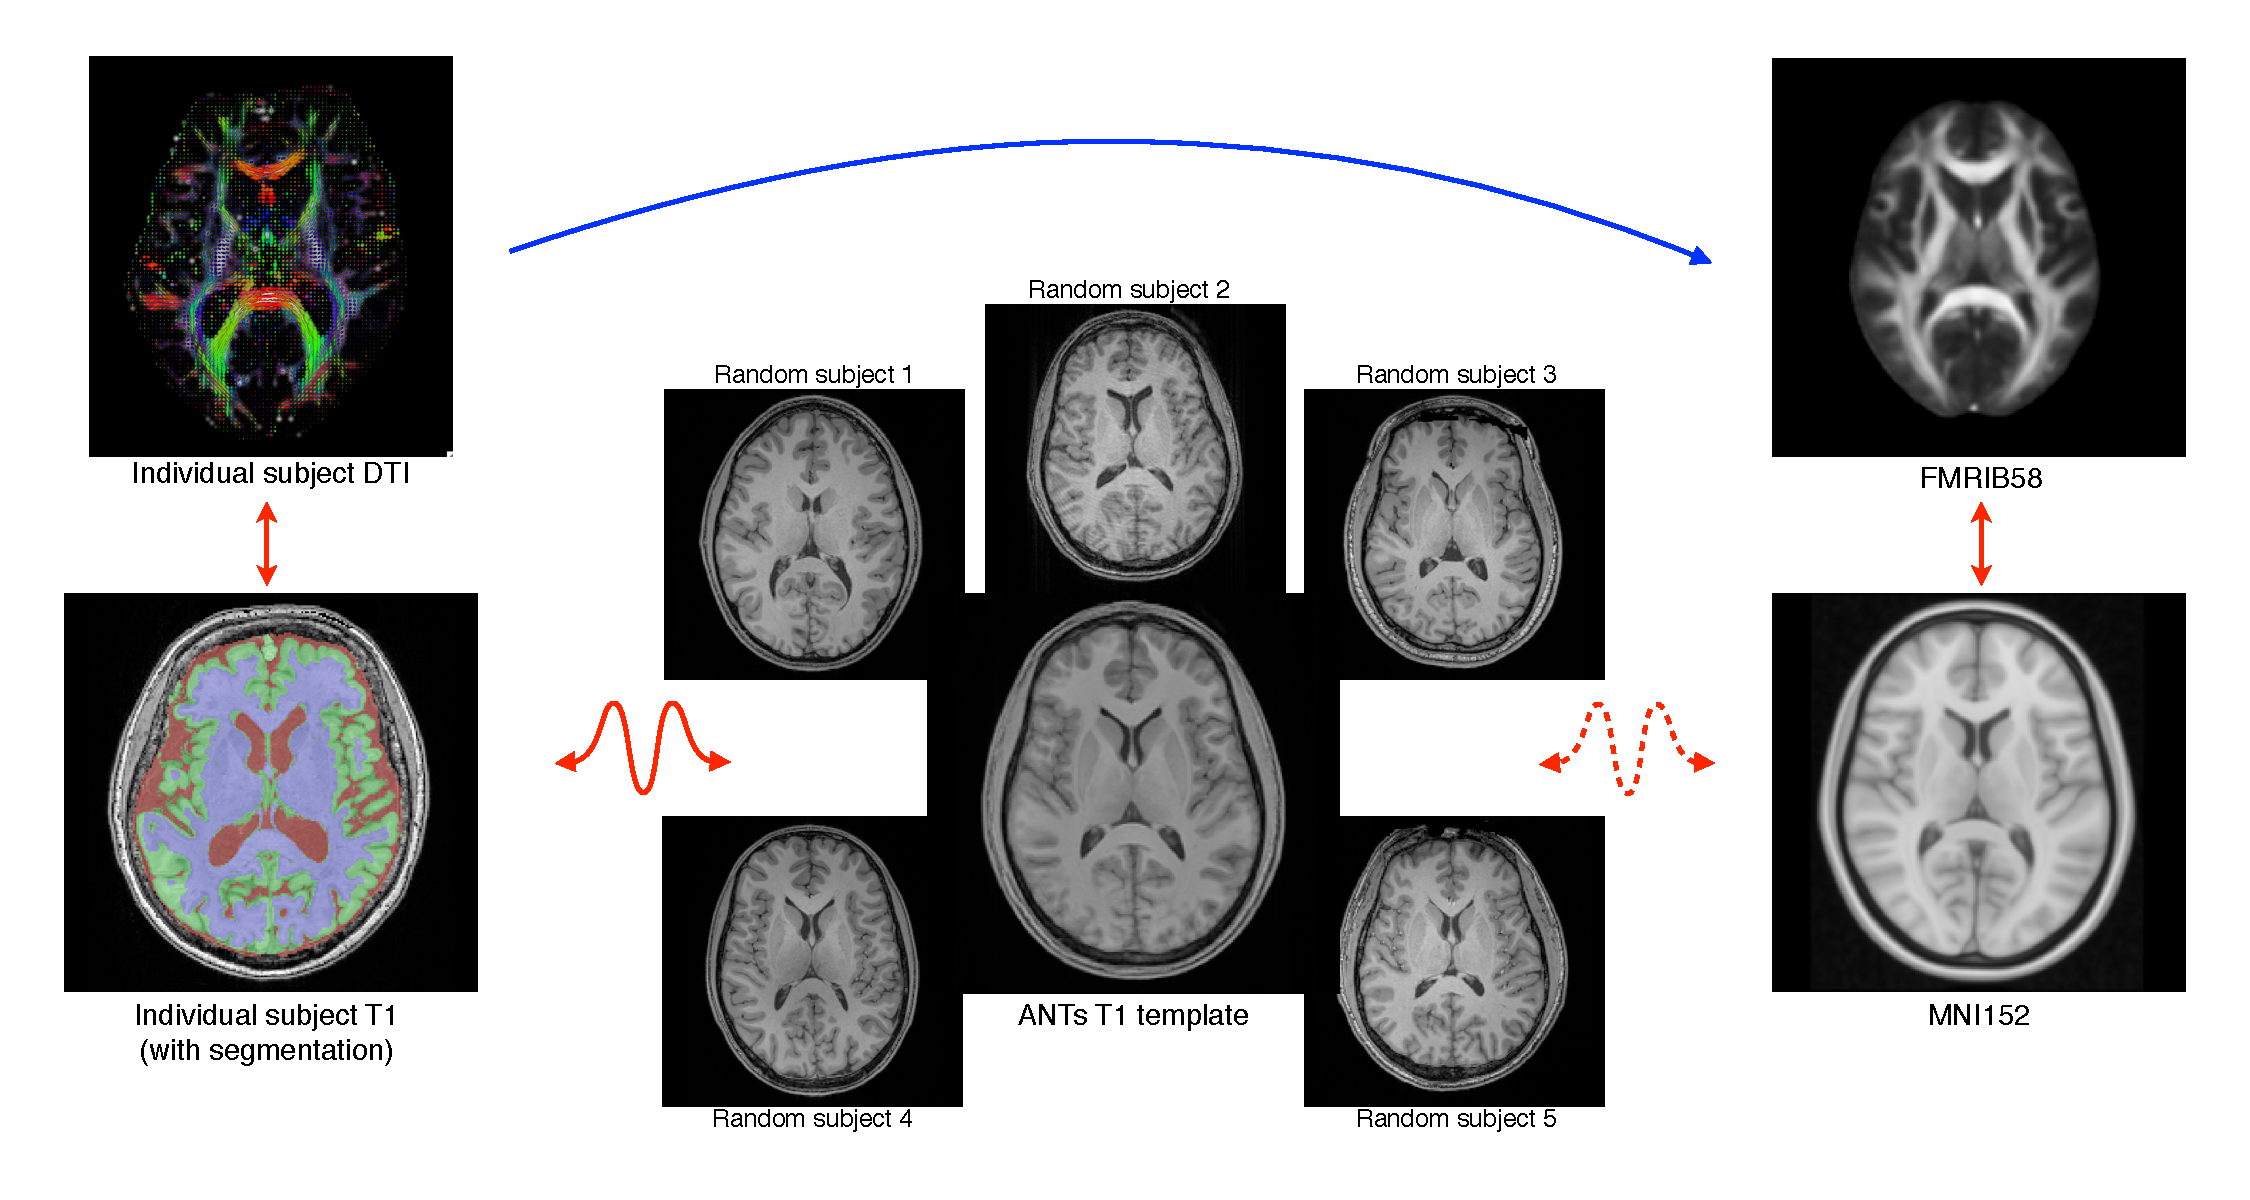
\includegraphics[width=170mm]{workflow.pdf}
%  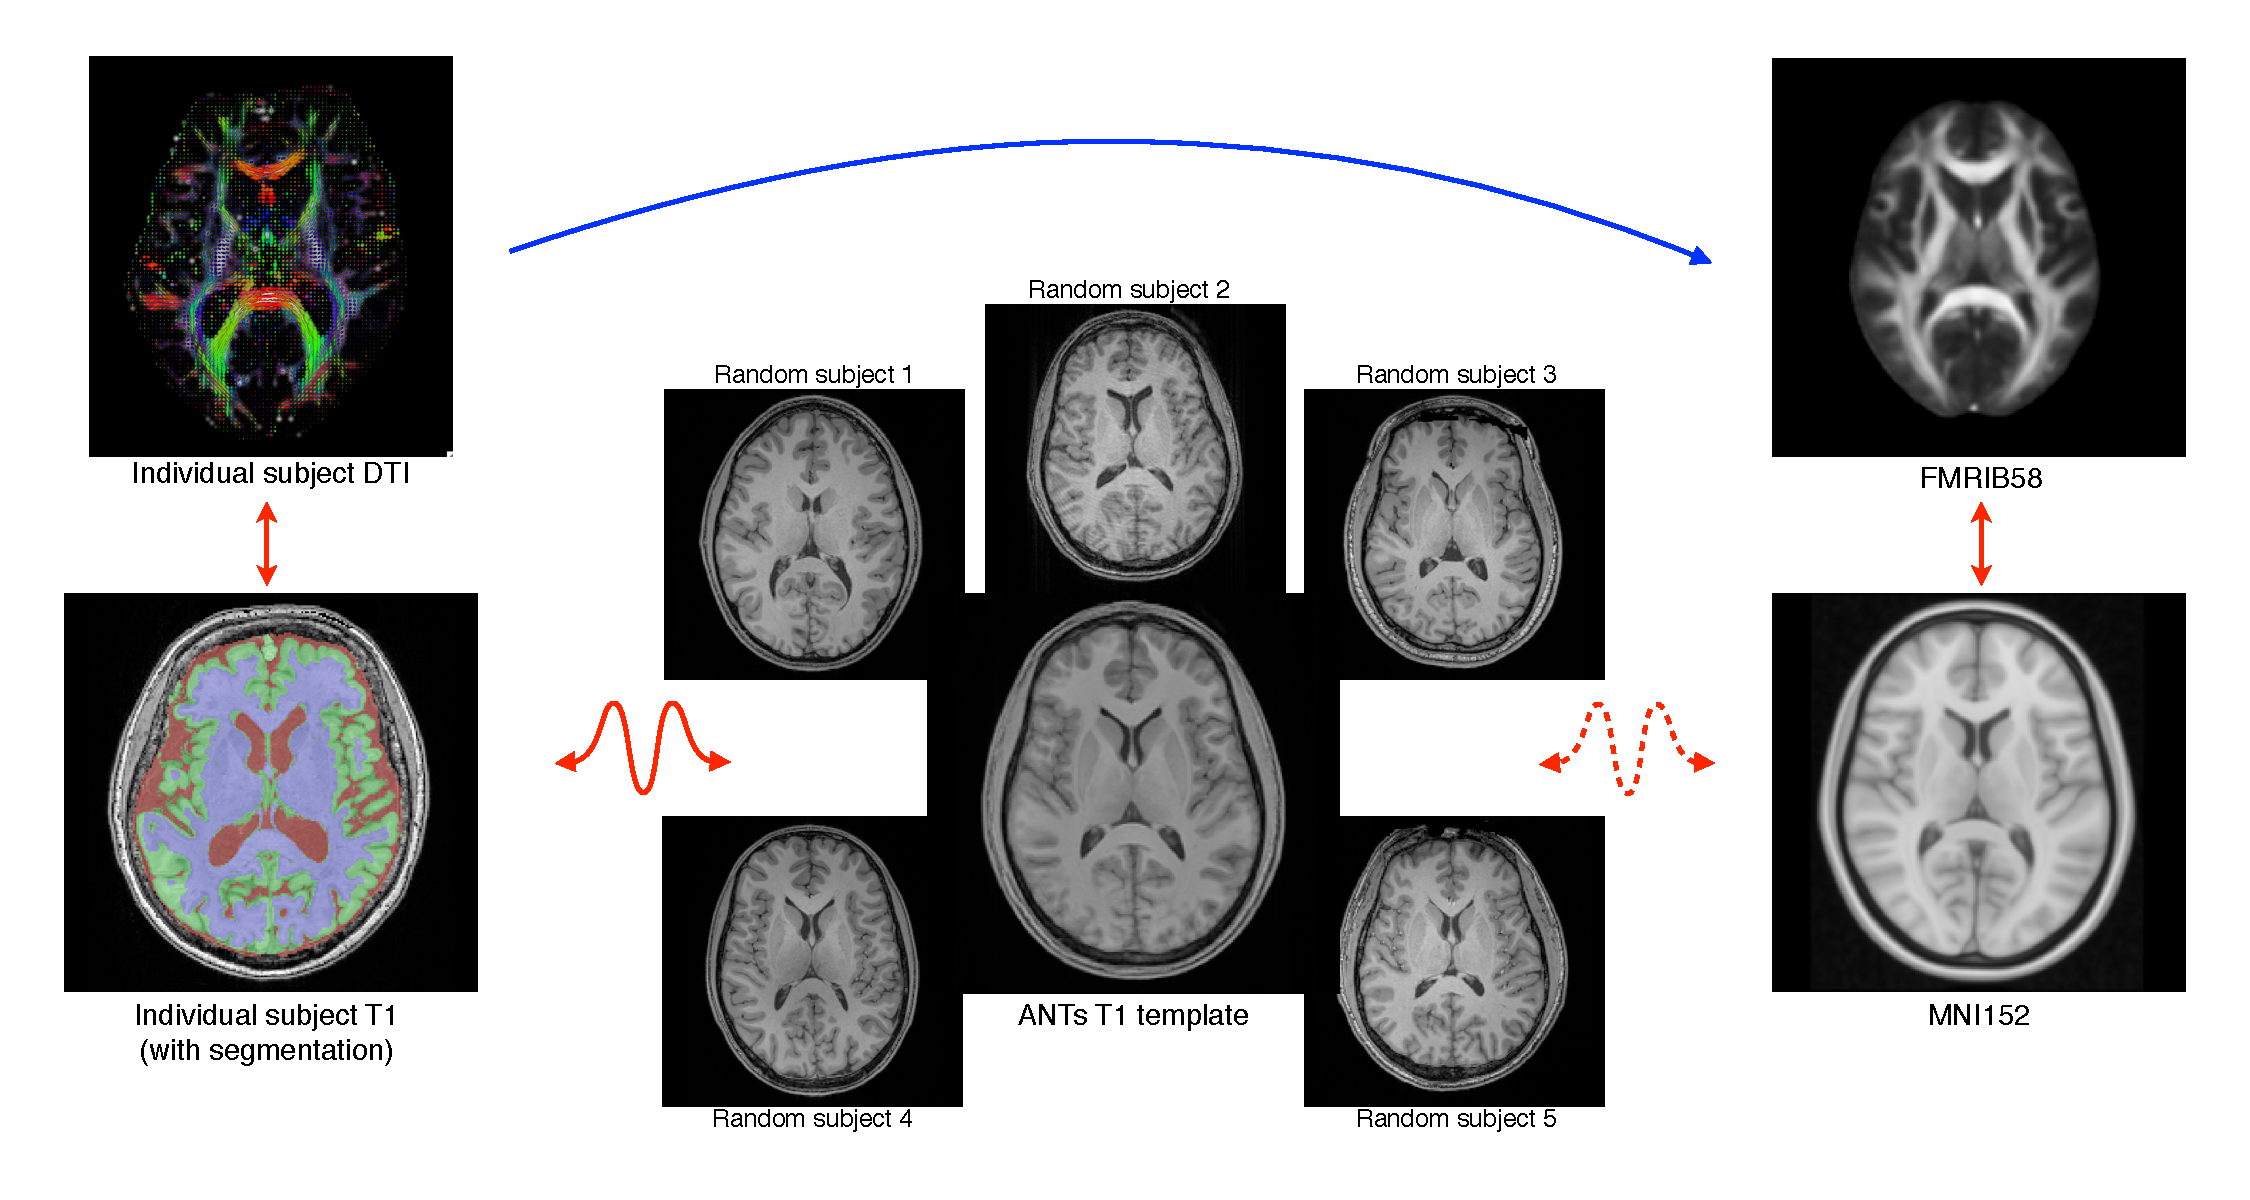
\includegraphics[width=130mm]{workflow.pdf}
\end{tabular}
\caption{Possible ANTs-based TBSS workflow using SyGN.  In contrast to standard TBSS in which an individual subject's FA is registered to the FMRIB58 template
(transform represented with the blue arrow), our proposed modification first constructs an ANTs optimal anatomical template as illustrated in the center of the figure.  Each FA image is then rigidly mapped, with distortion correction, to the individual T1 using the white matter mask as shown on the left.  The individual T1-weighted image is then nonrigidly registered to the anatomical template.  Optionally, one can register the T1 template to the MNI152 template which resides in the same space as the FMRIB58 template.  Thus, the composite transform, carefully constructed without any FA-to-FA image registration, can take an individual subject's FA map (or other DTI-derived measure) to the desired standardized coordinate system.    }
\label{fig:workflow}
\end{center}
\end{figure*}



In general, normalization to a standard coordinate system to
reduces intersubject variability in population studies.  Various
approaches exist for determining the normalized space such as selection
of a pre-existing template based on a single subject, e.g. the Talairach
atlas \citep{Talairach1988}, or a publicly available averaged group of
subjects, e.g. the MNI \citep{Collins1994} or ICBM \citep{Mazziotta1995}
templates.  
%One challenge with standard templates is that they may inadvertantly bias one's results by enabling better normalization of subjects to which the template is more similar.  This issue is exacerbated when dealing with populations that have high variance (e.g. due to disease) and/or when one's normalization method is low-dimensional (not flexible enough to capture large shape differences). 
Population-specific templates (or optimal templates) alleviate some of
these issues by deriving a most representative image from the population
\citep{Good2001}.  Large deformation registration algorithms also reduce
this confound by being less sensitive to the deformation distance
between subject and target.  Some approaches combine both advantages,
for instance, the diffeomorphic approach of Joshi et al. employs the
SSD metric and a shape distance to bring the subject group of images
into alignment \citep{Joshi2004}.  Variants
include extension to multiple modalities \citep{Lorenzen2006} and small deformations
\citep{Geng2009}.  These approaches iteratively minimize group difference in ``congealing''
towards a representative image template \citep{Learned-Miller2006}.
In contrast, Avants et al. explicitly model the geometric component of the 
normalized space during optimization.  Coupling the intrinsic symmetry of 
SyN pairwise registration \citep{Avants2011} and an
optimized sharpening/averaging of the template appearance, Symmetric Group
Normalization (SyGN) is a powerful framework for producing optimal population-specific
templates \citep{Avants2010} with arbitrary similarity metric choice. 

%Given a set of representative images, 
%$\{I_1, I_2, \ldots, I_M\}$, optimization involves finding the set of paired
%diffeomorphic transformations, $\left\{\left(\phi^1_1, \phi^1_2\right), 
%\left(\phi^2_1, \phi^2_2\right), \ldots, \left(\phi^M_1, \phi^M_2\right) \right\}$,
%the optimal template appearance, $J^*$, and corresponding coordinate system, $\psi(\mathbf{x})$,
%which minimize the following cost function:
%\begin{align}
%  \sum_{m=1}^M \left[
%    D\left( \psi(\mathbf{x}), \phi^m_1(\mathbf{x}, 1) \right) + 
%    \Pi \left( I_m\left(\phi^m_2(\mathbf{x}, 0.5) \right), J^*\left(\phi^m_1(\mathbf{x}, 0.5) \right) \right)
%    \right]
%\end{align}
%where $D$ is the diffeomorphic shape distance, 
%\begin{align}
%  D\left(\phi(\mathbf{x}, 0), \phi(\mathbf{x}, 1)\right) = \int_{0}^1 \| v(\mathbf{x}, t) \|_L dt, 
%\end{align}
%dependent upon the choice of the linear operator, $L$, and
%$v$ is the diffeomorphism-generating velocity field, 
%\begin{align}
%  v\left(\phi(\mathbf{x}, t), t \right) = \frac{d\phi(\mathbf{x}, t)}{dt},\,\,\, \phi(\mathbf{x}, 0) = \mathbf{x}.
%\end{align}
%$\Pi$ is the choice of similarity metric, often cross-correlation \citep{Avants2008a}, calculated in the 
%virtual domain midway between each individual image and the current estimate of the template. 
%
%With initial assignment of $\left\{\left(\phi^m_1, \phi^m_2\right)\right\}$ and $\psi(\mathbf{x})$ 
%to identity, iterative optimization
%involves estimating the pairwise transformations, estimation of the optimal template appearance, and 
%updating $\psi(\mathbf{x})$ by averaging the current estimate of $\left\{\phi_1^m\right\}$.  Additional details are given in \cite{Avants2010}.  
%For the interested reader, a set of scripts has been created and is distributed with the ANTs library for facilitating template creation.

Our proposed workflow applied to anatomically-based population normalization is illustrated in Fig. \ref{fig:workflow}.  Instead of direct FA-to-FA registration, our ANTs-based modification can be described as follows:

\begin{enumerate}
  \item Build the anatomical template from  the population sample or sample subset using SyGN as described in
  the previous section.
  \item If only using a sample subset for template creation, register the remaining
        anatomical data to the template and save the resulting transformation for each         
        subject indexed by $i$ (i.e. $\mathcal{T}^i_{template}$).
  \item Find the optimal transformation from each
        subject's FA to the anatomical template:
  \begin{enumerate}
  \item For each anatomical image, segment the white matter (in ANTs, one can use N4 bias correction \citep{Tustison2010} and Atropos $n$-tissue segmentation \citep{Avants2011a}).
  \item Rigidly transform each subject's average DWI to the bias-corrected anatomical image ($\mathcal{R}^i_{dwi}$).
  \item Perform distortion correction on the FA to anatomical mapping 
        by localized nonrigid registration
        of rigidly transformed FA map ($=\mathcal{R}^i_{dwi} \mathrm{FA}$) using
        the white matter mask obtained in step 3(a) ($\mathcal{T}^i_{FA}$).
  \item For each subject, concatenate the transforms which maps each
        subject's FA to the template ($\mathcal{T}^i_{total} = \mathcal{T}^i_{template} \circ 
        \mathcal{T}^i_{FA} \circ \mathcal{R}^i_{dwi} \mathrm{FA}$).
  \item Warp each subject's FA map to the template using $\mathcal{T}^i_{total}$.  
  Equivalently, one could warp the mean diffusion (MD), axial diffusion (AD) or any 
  other scalar derivable from DTI to the template.  
%  One other detail is that we prefer to warp the subject's DTI to 
%  the template and then, in template space, derive the scalar images of interest.  
  \end{enumerate}      
%  \item Perform the remaining portions of the standard TBSS pipeline:
%    \begin{enumerate}
%      \item Create the mean FA image from all template-aligned FA images.
%      \item Produce the white matter skeleton from the mean FA image.
%      \item Create skeleton distance map and project all FA data onto the skeleton.
%      \item Run the statistical analysis.
%    \end{enumerate}
\end{enumerate}
%The next section compares this framework to FA-based normalization strategies with respect to both a patient-control study and a study of gender effects in a control population.  


\subsection{Imaging Data}

\subsubsection{NKI/Rockland Data for Generation of the Simulated DTI Gender Cohort}
Data from the first 14 weeks of prospective data-sharing initiative sponsored by the 1000 Functional Connectomes Project (FCP)%
\footnote{
In support of open science, the 1000 Functional Connectomes Project (FCP---http://fcon\_1000.projects.nitrc.org) 
was initiated on December 11, 2009 by various members of the MRI community \citep{Biswal2010}.  Motivated by the absence of neuroimaging data for research, this initiative seeks to form collaborative partnerships with imaging institutions for sharing well-documented multi-modal image sets accompanied by phenotypic data.  Commitments from institutions such as the NYU Institute for Pediatric Neuroscience and the Nathan Kline Institute (NKI)--Rockland have resulted in prospective data repositories
currently distributed to the public via the Neuroimaging Informatics Tools and Resources Clearinghouse (NITRC---http://www.nitrc.org).
}
were downloaded on January 15, 2011 comprised of 74 subjects (average age in years: 32.4 $\pm$ 17.8).  
Due to various issues (e.g. lack of corresponding T1 image, failed DTI reconstruction, and age matching requirements) only 62 subjects (21 females and 41 males).  Each imaging session for each subject produced a 64-directional diffusion tensor imaging scan (parameters: conventional single-shot spin echo
EPI pulse sequence, TR = 10000 ms, TE = 91 ms, axial acquisition, 
voxel size = $2 \times 2 \times 2$ mm$^3$) and a T1 anatomical scan (parameters:  TR = 2500 ms, b = 1000 s/mm$^2$ for each direction, 58 contiguous slices of 2.0 mm thickness,
TI = 1200 ms, TE = 3.5 ms, flip angle = 8$^\circ$, 192 contiguous slices of 
1.0 mm thickness, FOV = 256 $\times$ 256 mm$^2$, and voxel size = 1 mm$^3$).  Images were anonymized including defacing of the T1 images prior to upload. Diffusion tensor data associated with each of the following data sets were reconstructed from the diffusion weighted sequences using Camino%
\footnote{
http://camino.org.uk/
}---an open source toolkit for diffusion MRI processing and 
analysis \citep{Cook2006} in combination with ANTs-based 
registration for motion correction of the DTI sequence.


\subsubsection{Diffuse Traumatic Brain Injury Data}

The TBI data used in this study is part of a larger effort investigating the relationship between various neuroimaging indices and cognitive and functional abilities in long-term survivors of TBI (principal investigator: John Whyte). A more detailed data description can be found in \cite{Avants2008}. The following is a brief description relevant to our particular study.  
17 controls and 16 patients with TBI were used for the analysis presented in this work.  Each patient had a history of non-penetrating traumatic brain injury 
of at least moderate severity defined by significant and well-documented
loss or alteration of consciousness following injury in addition to meeting
several other exclusionary criteria.  The healthy volunteers were matched in terms of age, gender, ethnicity, handedness, and years of education.
High resolution T1-weighted anatomic images were obtained using a 3D MP-RAGE 
imaging sequence with the following acquisition parameters: TR = 1620 ms, 
TI = 950 ms, TE = 3 ms, flip angle = 15$^\circ$, 160 contiguous slices of 
1.0 mm thickness, FOV = 192 $\times$ 256 mm$^2$, matrix = 192 $\times$ 256, 
1NEX with a scan time of 6 minutes, and voxel size = 1 mm$^3$.  30-directional
DTI images were also obtained. Diffusion tensor data were reconstructed using Camino.

\subsection{Simulated DTI Gender Cohort Creation}

\begin{figure}
\begin{center}
\begin{tabular}{cc}
  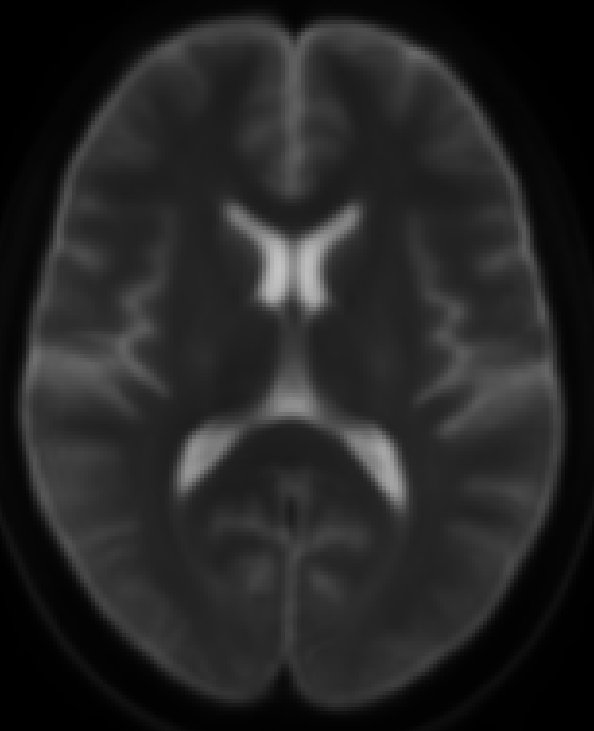
\includegraphics[width=41mm]{B0Average_slice85.png} & 
  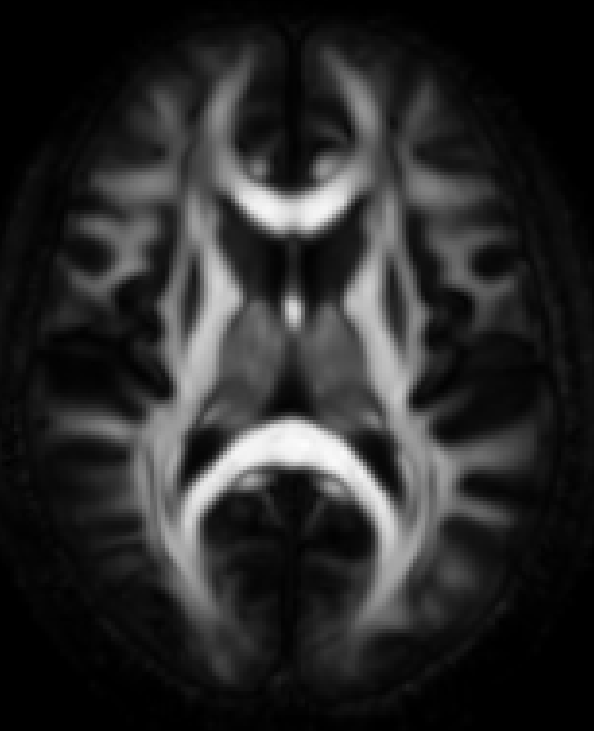
\includegraphics[width=41mm]{DTIAverageFA_slice85.png} \\
  (a) & (b) 
\end{tabular}
\caption{Mid-axial slice of the (a) average b0 image and (b) FA image derived from the DTI atlas used
to create the simulated gender data sets.}
\label{fig:simulated}
\end{center}        
\end{figure}


To provide realistic ground truth FA data, we implemented 
the work of Van Hecke et al. \cite{van-hecke2009} which 
we have also made available to the public
\cite{Tustison2011}.%
\footnote{
http://hdl.handle.net/10380/3315
}  
Given an input DTI atlas, b0 image, scheme file indicating
the gradient directions, and 
a cohort of aligned DTI data (to model intersubject variability), the
user is able to create 
simulated data sets with specified pathology and Rician noise.
For the simulated experiments described in the next section we
created a T1 template from 30 randomly chosen T1 images.  The
template was then registered to the MNI152 template.  
The remaining 32 T1 images were then registered to the
template.  Each DTI and b0 image was mapped to the MNI152 map as 
described above using the T1 to MNI composite mapping.  DTI 
were reoriented using the PPD method \cite{alexander2001}.  The 62
aligned DTI were averaged using the log-euclidean framework 
\cite{arsigny2006} to create the DTI atlas.  Similarly, the 62 aligned
b0 images were averaged to create the representative b0 image
for simulated DTI creation.  The derived FA and b0 images are shown in 
Fig. \ref{fig:simulated}.  An FA mask was created by thresholding 
the FA image of the DTI atlas at 0.2.


The 41 aligned male DTI were used to generate 18 ``Control'' 30-direction
diffusion-weighted images
with no simulated noise nor pathology.  Similarly, the 21 aligned female
DTI were used to generate 19 ``Experimental'' diffusion-weighted images.  
DTI were reconstructed using Camino which were then use to create
individual FA images were
created from the DTI images to use in the simulated experiments.
The number of subjects in each
group was chosen based on the median control and experimental
subject numbers from a sampling of FA studies.  


%Drawing upon recent
%literature, Van Hecke et al. point out that white matter pathology,
%typically due to demyelination and axonal degeneration, is manifest 
%in DTI by a decrease in longitudinal diffusivity and an increase
%in transverse diffusivity.  This change corresponds to a decrease
%in the first eigenvalue and increase in the second and third
%eigenvalues, respectively, of the diffusion tensor.  These values
%are specified via the mask option so that user-specified pathologies
%can be tailored to different regions. One decision that
%we made, which is not explicit in the text was how to
%distribute the increase in eigenvalues 2 and 3 in the case
%of pathology.  To address this omission, we assumed a constant
%ratio before and after increasing the eigenvalues corresponding
%to transverse diffusion.


%We have included the short command
%line help in Listing 1 for the interested reader who would like to 
%reproduce our results.  
%
%\begin{figure}
%\lstsetcpp
%\begin{lstlisting}
%COMMAND: 
%     CreateDTICohort
%
%OPTIONS: 
%     -d, --image-dimensionality 2/3
%     -a, --dti-atlas inputDTIAtlasFileName
%     -x, --label-mask-image maskImageFileName
%                            lowerThresholdValue
%     -n, --noise-sigma <noiseSigma=18>
%     -p, --pathology label[<percentageChangeEig1=-0.05>,
%             <percentageChangeAvgEig2andEig3=0.05>,
%             <numberOfVoxels=all or percentageOfvoxels>]
%     -w, --dwi-parameters [B0Image,directionFile,bvalue]
%                          [B0Image,schemeFile]
%     -r, --registered-population dtiFileNames.txt
%     -o, --output [outputDirectory,fileNameSeriesRoot,
%             <numberOfControls=10>,
%             <numberOfExperimentals=10>]
%     -h 
%     --help 
%\end{lstlisting} 
%\end{figure}

















\section{Results}
%Results should be clear and concise.

\subsection{Simulated data set} 


\begin{figure*}
\begin{center}
\begin{tabular}{cc}
  \includegraphics[width=86mm]{ISV_SpeSenAlreadyAligned.pdf} &
  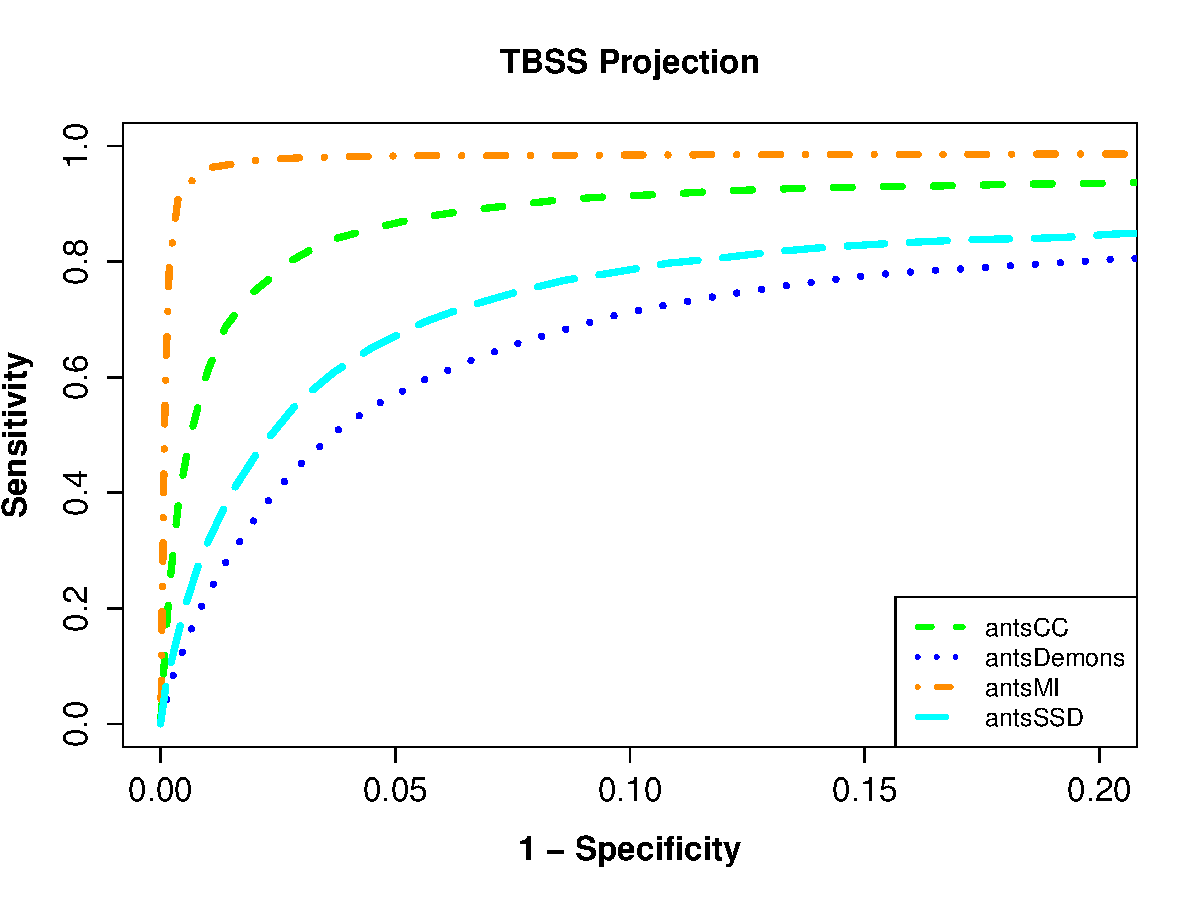
\includegraphics[width=86mm]{ISV_SpeSen_projectionAlreadyAligned.pdf}
\end{tabular}
\caption{ROC curves plotting $(1 - specificity)$ vs. $sensitivity$ for the
different simulated experiments for both (a) voxelwise analysis over the
entire FA mask and (b) using TBSS projections onto the mean FA skeleton.
Degree of locality and correspondence to 
Eqn. (\ref{eq:variance}) resulted in performance disparity between the
different metrics.  Since SSD and the SSD-like Demon's formulation 
minimize voxelwise group variance, we see the greatest bias in those 
two metrics.  In contrast, MI and CC are less susceptible to bias with
MI performing quite well.  Comparing voxelwise and projection results, 
it is apparent that the TBSS projection strategy only slightly improves 
the effects of bias for the simulated data.
}
\label{fig:simulated_plots}
\end{center}        
\end{figure*}

To demonstrate the significance of circularity bias on voxelwise 
analysis and to demonstrate its correspondence with different
common similarity metrics, we used the simulated DTI images 
described earlier to quantify such effects in FA.
Since each simulated DTI and derived FA map was generated in the
MNI152 template space, the cohort is already anatomically
aligned.  However, as described in the introduction, localized
image registration using common similarity metrics drive the 
alignment towards minimizing local intensity differences (not necessarily
anatomical differences) thereby
inducing false positives.  To test this, we applied ANTs registration
using default regularization and transformation parameters with
four common similarity metrics:  neighborhood cross-correlation (CC), 
Demons, mutual information (MI), and sum of squared differences (SSD).
We limited optimization to 10 iterations at the full resolution 
level.%
\footnote{
Specifically, the ANTs command line parameters common to each metric were:
{\tt -i 10 -t SyN[0.25] -r Gauss[3,0]}.
}
Since neither noise nor pathology was introduced, only the differences
associated with the gender cohort modeling is responsible for driving
the registration.

Voxelwise analysis included performing Student's t-test within the
DTI masked region (FA $\geq 0.2$) for both the ground truth (i.e.
anatomically aligned) data set and performing the same calculations
for each of the four registration scenarios.  We used a significance
level cutoff of $p = 0.05$ to determine ground truth significant
voxels in the already aligned data set.  We then varied the 
significance level cutoff for each of the registered data sets to plot
the corresponding ROC curves given in Fig. \ref{fig:simulated_plots}.
Visual comparison of the significant regions associated with the 
voxelwise analysis for ground truth data and with the Demons registration data for
$p \leq 0.05$ shown in Fig. \ref{fig:simulated_significance} demonstrates 
the potential severity metric choice can have on results.

We also performed a similar assessment
where instead of performing voxelwise calculations over the entire
white matter mask, we performed the FA skeleton projection characteristic
of TBSS using the relevant portions of the TBSS scripts found in the 
FMRIB software library (FSL).%
\footnote{
http://www.fmrib.ox.ac.uk/fsl/
}
The FA 
image produced from the
DTI atlas was used to produce a common skeleton for all comparisons.
The associated ROC curves are given
in the right plot of Fig. \ref{fig:simulated_plots}.  Although projection
does have slightly ameliorating effects, the associated bias is still 
significant across certain metrics.  

Despite the experimental set-up ensuring anatomical alignment in the
ground truth data, the resulting bias effects accord with our earlier 
description of the problem with these similarity metrics and direct
FA-to-FA template normalization.  
Whereas MI shows very little effects of bias due to it's statistical
formulation and relative non-locality, the SSD and SSD-like Demons
metrics are formulated such that they explicitly minimize voxelwise
group variance and thus induce such bias effects.

It should be noted that all the effects described are absent
any multiple comparisons corrections or smoothing prior to statistical
testing.  Although such techniques can minimize 
or even possibly eliminate these detrimental confounds, our contention
is (and these results demonstrate) that normalization choices can significantly
impact the results prior to any such
post hoc corrections and scientific best practices dictate that, where possible, 
experimental adjustments eliminating or minimizing potential sources of bias should
be made prior to experimental execution and analysis.  




\begin{figure}
\begin{center}
\begin{tabular}{cc}
  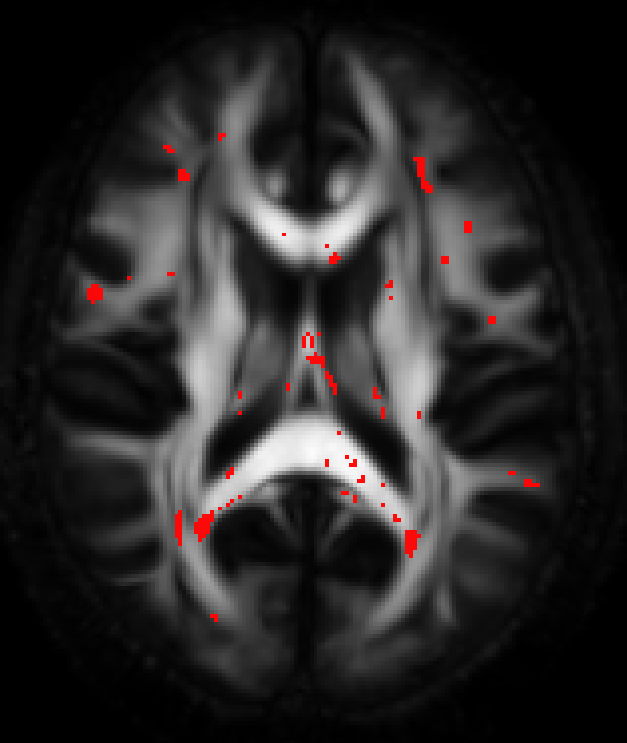
\includegraphics[width=41mm]{no_registration_voxelwise_slice90.png} &
  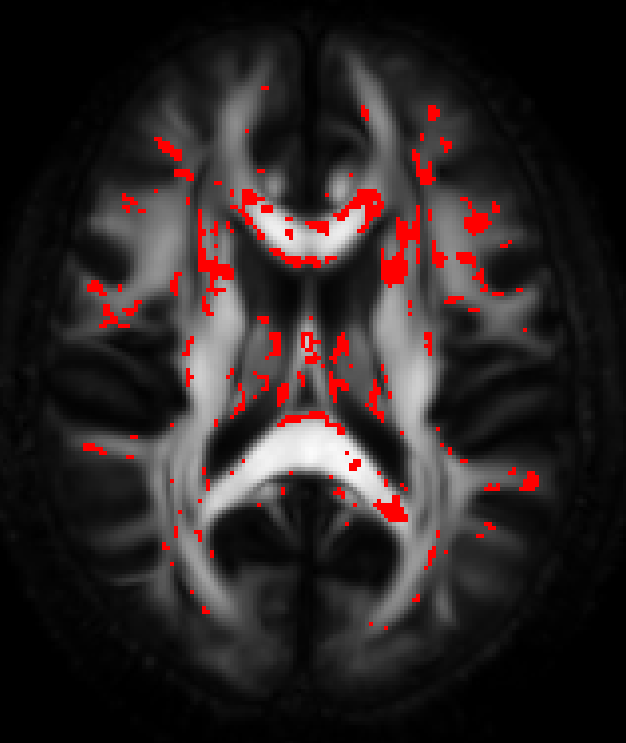
\includegraphics[width=41mm]{demons_voxelwise_slice90.png} \\
  (a) & (b)
\end{tabular}
\caption{(a) Mid-axial slice of the DTI atlas-derived FA map where the 
significant differences ($p < 0.05$) between control (male) and 
experimental (female) groups are labeled in red.  (b) Same mid-axial 
slice showing an increase in significant regions following ANTs 
registration employing the Demons metric.
}
\label{fig:simulated_significance}
\end{center}        
\end{figure}



\subsection{TBI Cohort} 



%\begin{figure*}
%\begin{center}
%\begin{tabular}{c}
%  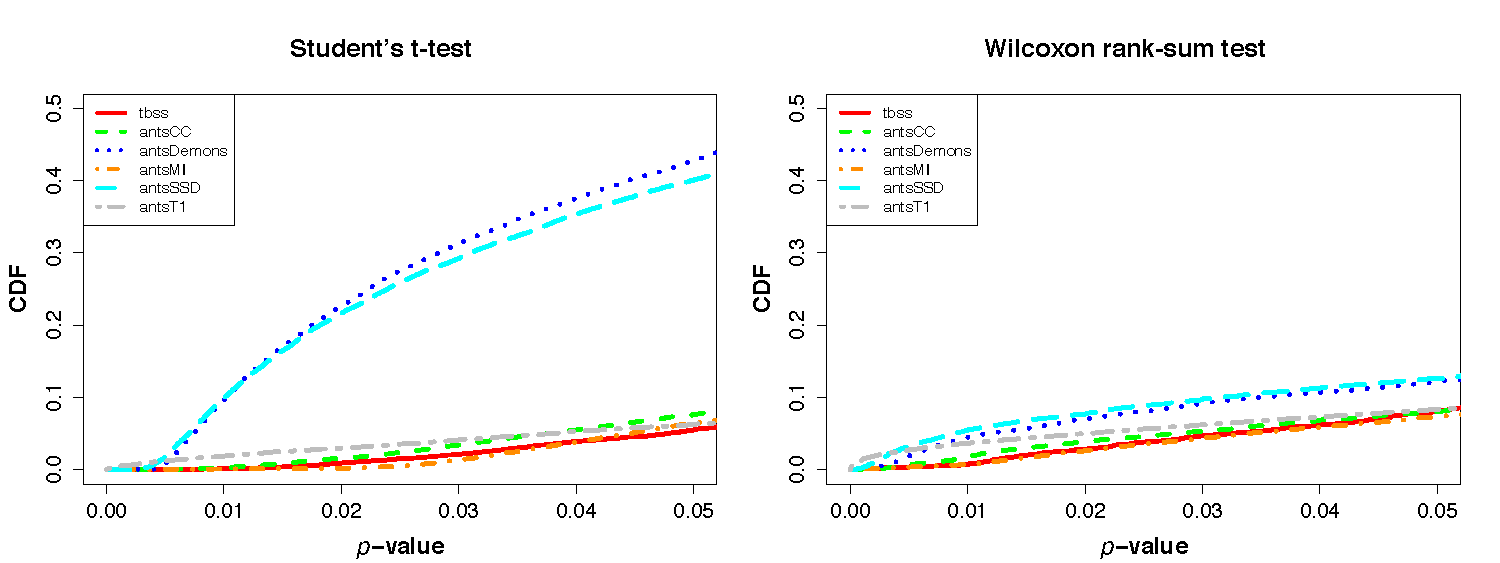
\includegraphics[width=180mm]{tbiTesting.pdf}
%\end{tabular}
%\caption{Student's $t$-test and the nonparametric Wilcoxon rank-sum test results (one-tailed, $\alpha = 0.95$) for the TBI FA data aligned to the FMRIB58 template adjusted for multiple comparisons (FDR).  Elevated statistical power is seen in the $t$-test with the similarity metrics with the most correspondence to Eqn. (\ref{eq:variance}), namely the SSD and Demons metric which shrinks drastically for the Wilcoxon rank-sum test.  Results for the other metrics including TBSS and the T1 template-based strategy (``antsT1'') remain fairly stable between the two tests.    TBSS and the 4 ANTs metric
%results were all obtained using direct registration involving subject FA and the FMRIB58 template.  The antsT1 results were also obtained in FMRIB58 space but the following transformation composition: subject FA $\rightarrow$ subject T1 $\rightarrow$ group T1 template $\rightarrow$ 
%common T1 template $\rightarrow$ MNI152 (FMRIB58) template.    }
%\label{fig:tbi_testing}
%\end{center}        
%\end{figure*}

Even under ideal conditions (i.e. no noise, no pathology, simple modeling of 
intersubject variation, and precise anatomical alignment), the simulated
data demonstrated the presence of circularity bias that varied with similarity
metric.  In this section, we use data that was analyzed in \cite{Stone2011}
and show how bias is potentially manifested in real data. 

We constructed a patient template and a control template from the 
T1-weighted images of the two groups.  These two 
templates were then used to create a third common template.  
To compare with TBSS normalization, the common template was
registered to the MNI152 template.  Thus, the transformation
which takes the FA image of an individual subject to the FMRIB58
template is the composition of transforms: 
subject FA $\rightarrow$ subject T1 $\rightarrow$ group T1 template $\rightarrow$ 
common T1 template $\rightarrow$ MNI152 (FMRIB58) template.
We evaluated this strategy relative to direct FA-to-FA
ANTs registration with the common similarity metrics used in
the simulated data example described earlier.
Standard TBSS alignment was also performed.  

Cumulative distribution functions (CDF) of the $p$-values (one-tailed, $\alpha = 0.95$)
over the entire FA mask (FA $\geq 0.2$) for the different normalization
strategies are shown in Fig. \ref{fig:tbi_testing}.
A bias which (falsely) decreases $p$-values will demonstrate a left-shifted
CDF. 
  The Demons and SSD power decreases while the others
remain fairly similar.  Interestingly, the ANTs template-based approach
trends towards better performance relative to the remaining 3 strategies.
It should be noted that although TBSS uses the SSD metric, the fixed and moving images are smoothed and subsampled even at the highest resolution level which substantially decreases the local effect of the metric.

%This is very much related to earlier findings in that strategies evincing
%greater alignment, as quantified by the CV,
%will trend towards smaller variance thus exhibiting a left-shifted
%CDF.  


%Similar to previous findings with the simulated data, the SSD and 
%Demons metric show an elevated effect using the Student's 
%$t$-test over the other alignment protocols which all exhibit similar 
%strength. 


\begin{figure}
\begin{center}
\begin{tabular}{c}
  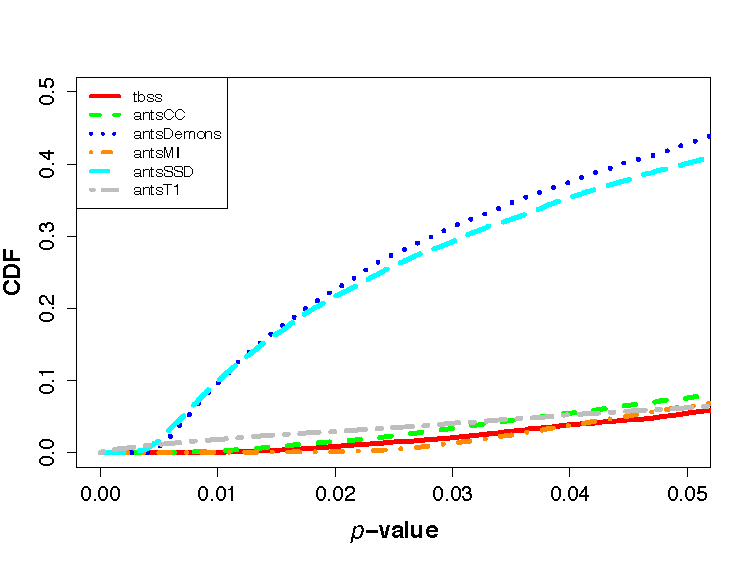
\includegraphics[width=85mm]{tbittest.pdf}
\end{tabular}
\caption{Student's $t$-test results (one-tailed, $\alpha = 0.95$) for the TBI FA data aligned to the FMRIB58 template adjusted for multiple comparisons (FDR).  Elevated statistical power is seen in the $t$-test with the similarity metrics with the most correspondence to Eqn. (\ref{eq:variance}), namely the SSD and Demons metric.  Results for the other metrics including TBSS and the T1 template-based strategy (``antsT1'') remain fairly stable between the two tests.    TBSS and the 4 ANTs metric
results were all obtained using direct registration involving subject FA and the FMRIB58 template.  The antsT1 results were also obtained in FMRIB58 space but the following transformation composition: subject FA $\rightarrow$ subject T1 $\rightarrow$ group T1 template $\rightarrow$ 
common T1 template $\rightarrow$ MNI152 (FMRIB58) template.  
}
\label{fig:tbi_testing}
\end{center}        
\end{figure}

The CDF of the voxelwise FA coefficient of variation (CV) of the aligned
images is shown for each case in Figure \ref{fig:tbi_cov}.  
The CV at each voxel is defined as the variance
divided by the mean over the population of FA values.  Thus,
those metrics which best minimize the voxelwise variance would
trend towards greater alignment as quantified by the CV.
Although direct FA-to-FA registration using ANTs with common
similarity metrics gives ``better alignment'' such alignment is 
produced at a cost of significant Type 1 errors.  Common subsampling and
smoothing strategies and local neighborhood metrics such as CC and MI reduce the 
Type 1 error problem (as evidenced in Fig. \ref{fig:tbi_testing}) 
but also show a decrease in alignment.  

Finally, qualitative assessment is provided in Fig. \ref{fig:meanFA} 
in which the mean FA image derived from the template-based approach
and the post-normalization component of the TBSS pipeline (Fig. \ref{fig:meanFA}(c)) 
is juxtaposed 
with the mean FA image produced by the TBSS pipeline alone (Fig. \ref{fig:meanFA}(a)).
The skeleton masks were produced by thresholding the skeleton values at 
FA $\geq 0.2$ and it would appear that the improved alignment produces 
a more extensive skeletal network for greater localization testing of 
significant differences, particularly in the outer white matter regions
(compare Fig. \ref{fig:meanFA}(b) and Fig. \ref{fig:meanFA}(d)).
%Given that TBSS is intrinsically a statistical method for finding local 
%differences, improved alignment would presumably provide increased regional sensitivity to differences.



\begin{figure}
  \begin{center}
\begin{tabular}{c}
  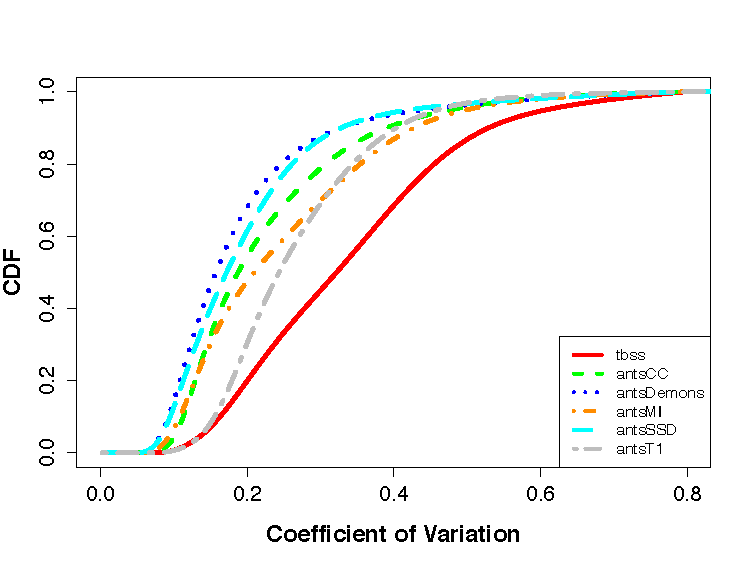
\includegraphics[width=85mm]{tbiCoV.pdf}
\end{tabular}
\caption{Comparison of the different alignment strategies in normalizing the TBI data to the FMRIB58 template.  Assessment is quantitated using the voxelwise CV of the FA.  TBSS and the 4 ANTs metric
results were all obtained using direct registration involving subject FA and the FMRIB58 template.  The curve denoted as ``antsT1'' was also obtained in FMRIB58 space with the following transformation composition: subject FA $\rightarrow$ subject T1 $\rightarrow$ group T1 template $\rightarrow$ 
common T1 template $\rightarrow$ MNI152 (FMRIB58) template. }
\label{fig:tbi_cov}
\end{center}
\end{figure}

\begin{figure}
\begin{center}
\begin{tabular}{c}
  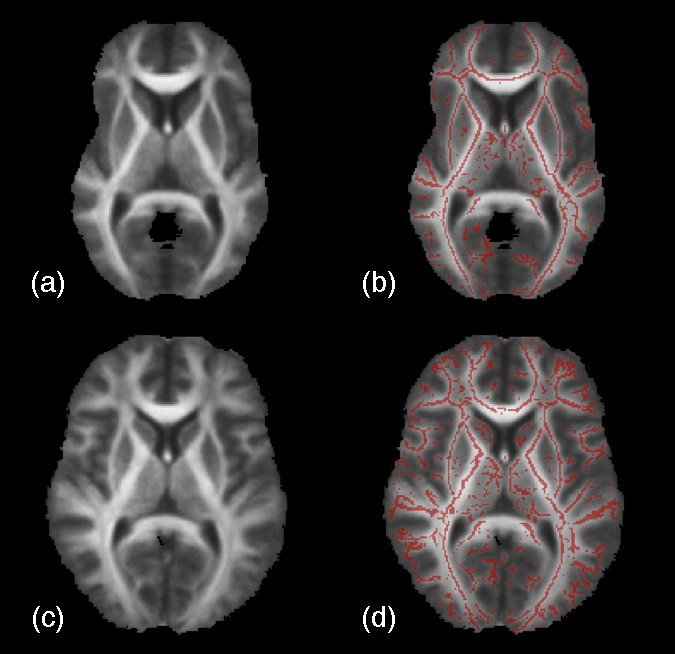
\includegraphics[width=85mm]{meanFA.pdf}
\end{tabular}
\caption{Qualitative comparison of mean FA images used in TBSS taken from the TBI data described in Section 2.  The mean FA image illustrated in (a) is created by mapping the sample FA population to the default FMRIB58 template which is the standard protocol for TBSS.  In comparison, the mean template represented in (c) is created from alignment of the population sample to the optimal T1 template as described in the paper. The respective skeleton masks in (b) and (d) are created by thresholding the resulting skeleton values $\geq 0.2$.  }
\label{fig:meanFA}
\end{center}
\end{figure}

%\section{Discussion}
%This should explore the significance of the results of the work, not repeat them. A combined Results and Discussion section is often appropriate. Avoid extensive citations and discussion of published literature.

\section{Discussion and Conclusions} 
Prior evaluation work using anatomically labeled
data indicates that mutual information, cross-correlation, Demons, and
SSD metrics are all capable of producing high quality anatomical
alignment (e.g. \citep{Klein2009}).  All of this work, though, compares
the quality of alignment at a relatively coarse scale of major gyri,
lobes and regions.  At the voxel level, it is nearly impossible to
determine the ground truth correspondence.  Indeed, there is no reason
to believe that subtle differences between a set of alignment
strategies (induced, in the experiments of this paper, by changing the
similarity metrics used in image registration) that all apparently
work well should be considered significant.  This work, however,
highlights a dramatic impact of similarity metric choice on detection
power in template-based FA studies.  Our contention is that this
dramatic ``improvement'' in detection power is not due to better
anatomical alignment.  Rather, it is a result of the
circularity/nonindependence of the normalization and statistical
estimation strategy.  Consequently, we recommend that future work
should take greater care when pairing the normalization strategy with
the statistical framework.  Furthermore, we recommend that researchers
should diligently seek to maintain independence between these two
critical stages of a population study.  That is, the features that
drive the minimization of a similarity metric should be independent of
the features that will be used in hypothesis testing.  In particular,
one should avoid combining the SSD metric for normalizing FA with
Student's $t$-test for FA differences.  A final point is that
cumulative distribution functions and other power assessment methods
cannot be regarded as meaningful comparison techniques in the presence
of normalization/statistical nonindependence.  Similar issues are
raised in \cite{Kriegeskorte2010}.

Caveats with our analysis include a lack of ground truth in the
clinical component of the study.   Additionally, we are not addressing
the biological plausibility of our results nor do we
intend to (in this paper) enter into discussion on the mechanisms of
TBI, gender difference, and DTI that may lead to the detected results.
Rather, we focus on the technical issue of circularity caused by
normalizing the image feature of interest with functions that maximize
the statistic used in hypothesis testing.  We also cannot argue that our analysis
invalidates previous studies in which circularity might be an issue.  
Finally, we do not address the very promising work concerning
whole tensor DTI normalization \citep{Zhang2007,Hecke2007}, DTI template-based
strategies \citep{Mori2009,Hecke2011}, or other related methods \cite{jbabdi2010}.  
%Although investigation is beyond the scope
%of this work, these whole-tensor approaches might provide the necessary
%anatomical information to overcome the deficiencies addressed in this
%work.

Instead, we encourage the community to
reexamine FA normalization and analysis methods and to consider the
potential confounds highlighted in this paper and others
\cite{Ridgway2008}.  Rank tests
provide a more conservative alternative as does the methodology
presented here based on T1 to DT intrasubject mapping and T1
normalization.  To our surprise, we could not find a prior publication that directly
addresses this issue.  Two reasons may be that the majority of
technical work using DTI has focused on more cutting-edge issues while
the clinical work using DTI is more concerned with generating
statistically significant results.  An additional reason may be that
only recently have toolkits emerged to enable easy comparison of
statistical techniques (via {\bf R} \citep{RDevelopmentCoreTeam2011}), normalization methods (ANTs), and
diffusion tensor processing (Camino).


%% The Appendices part is started with the command \appendix;
%% appendix sections are then done as normal sections
%% \appendix

%% \section{}
%% \label{}

%% References
%%
%% Following citation commands can be used in the body text:
%% Usage of \cite is as follows:
%%   \citep{key}          ==>>  [#]
%%   \cite[chap. 2]{key} ==>>  [#, chap. 2]
%%   \citet{key}         ==>>  Author [#]

%% References with bibTeX database:

\section*{Acknowledgments}
All visualizations were performed using ITK-SNAP%
\footnote{
http://www.itksnap.org/
}
\citep{Yushkevich2006} and
DTI-TK.%
\footnote{
http://www.nitrc.org/projects/dtitk/
}
We also gratefully acknowledge Dr. Niels van Strien of the Norwegian University of Science and Technology
who assisted in packaging the template construction algorithm in the very useful script \verb#buildtemplateparallel.sh#
which is publicly available in ANTs.

\section*{References}

\bibliographystyle{elsarticle-harv}
\bibliography{references}


%% Authors are advised to submit their bibtex database files. They are
%% requested to list a bibtex style file in the manuscript if they do
%% not want to use model1-num-names.bst.

%% References without bibTeX database:

% \begin{thebibliography}{00}

%% \bibitem must have the following form:
%%   \bibitem{key}...
%%

% \bibitem{}

% \end{thebibliography}


\end{document}

%%
%% End of file `elsarticle-template-1-num.tex'.
